\documentclass[%
crop,%
tikz,%
convert={outext=.svg,command=\unexpanded{pdf2svg \infile\space\outfile}},%
multi=false%
]{standalone}%
\usepackage[utf8]{luainputenc}%
\usepackage{xspace}%
\usepackage{amsmath}%
\usepackage{amssymb}%
\usepackage{mathrsfs}%
\usepackage{mathtools}%
\usepackage{siunitx}%
\usepackage[siunitx,european,straightvoltages]{circuitikz}%
\usetikzlibrary{calc,backgrounds}%
\DeclareMathOperator{\sign}{sign}%

% Ensembles
\let\C\relax
\newcommand{\R}{\ensuremath{\mathbb{R}}} % Réel
\newcommand{\N}{\ensuremath{\mathbb{N}}} % Entiers naturels
% \newcommand{\C}{\ensuremath{\mathbb{C}}} % Complexes
\newcommand{\B}{\ensuremath{\mathscr{B}}} % Bus électriques
\newcommand{\Ch}{\ensuremath{\mathscr{C}}} % Charges
\renewcommand{\L}{\ensuremath{\mathscr{L}}} % Lignes
\renewcommand{\P}{\ensuremath{\mathscr{P}}} % Phases

% Phases
\newcommand{\arm}{\ensuremath{\mathrm{a}}}%
\newcommand{\brm}{\ensuremath{\mathrm{b}}}%
\newcommand{\crm}{\ensuremath{\mathrm{c}}}%
\newcommand{\nrm}{\ensuremath{\mathrm{n}}}%
\newcommand{\trm}{\ensuremath{\mathrm{t}}}%
\newcommand{\abrm}{\ensuremath{\mathrm{ab}}}%
\newcommand{\bcrm}{\ensuremath{\mathrm{bc}}}%
\newcommand{\carm}{\ensuremath{\mathrm{ca}}}%
\newcommand{\anrm}{\ensuremath{\mathrm{an}}}%
\newcommand{\bnrm}{\ensuremath{\mathrm{bn}}}%
\newcommand{\cnrm}{\ensuremath{\mathrm{cn}}}%
\newcommand{\atrm}{\ensuremath{\mathrm{at}}}%
\newcommand{\btrm}{\ensuremath{\mathrm{bt}}}%
\newcommand{\ctrm}{\ensuremath{\mathrm{ct}}}%
\newcommand{\ntrm}{\ensuremath{\mathrm{nt}}}%
\newcommand{\abcrm}{\ensuremath{\mathrm{abc}}}%
\newcommand{\abcnrm}{\ensuremath{\mathrm{abcn}}}%

% Indices ou exposants
\newcommand{\cons}{\ensuremath{\mathrm{cons.}}}%
\renewcommand{\prod}{\ensuremath{\mathrm{prod.}}}%
\newcommand{\theo}{\ensuremath{\mathrm{th.}}}%
\newcommand{\const}{\ensuremath{\mathrm{const.}}}%

% Variables
\newcommand{\umax}{\ensuremath{U^{\max}}}%
\newcommand{\umaxnorm}{\ensuremath{U^{\max\,\text{norm.}}}}%
\newcommand{\umin}{\ensuremath{U^{\min}}}%
\newcommand{\uminnorm}{\ensuremath{U^{\min\,\text{norm.}}}}%
\newcommand{\unom}{\ensuremath{U^{\text{nom.}}}}%
\newcommand{\unomnorm}{\ensuremath{U^{\text{nom.}\,\text{norm.}}}}%
\newcommand{\uup}{\ensuremath{U^{\text{up}}}}%
\newcommand{\uupnorm}{\ensuremath{U^{\text{up}\,\text{norm.}}}}%
\newcommand{\uupprime}{\ensuremath{U^{\text{up}\,\prime}}}%
\newcommand{\udown}{\ensuremath{U^{\text{down}}}}%
\newcommand{\udownnorm}{\ensuremath{U^{\text{down}\,\text{norm.}}}}%
\newcommand{\udownprime}{\ensuremath{U^{\text{down}\,\prime}}}%
\newcommand{\smax}{\ensuremath{S^{\max}}}%
\newcommand{\pmax}{\ensuremath{P^{\max}}}%
\newcommand{\sproj}{\ensuremath{\underline{S^{\text{proj.}}}}}%
%
\begin{document}
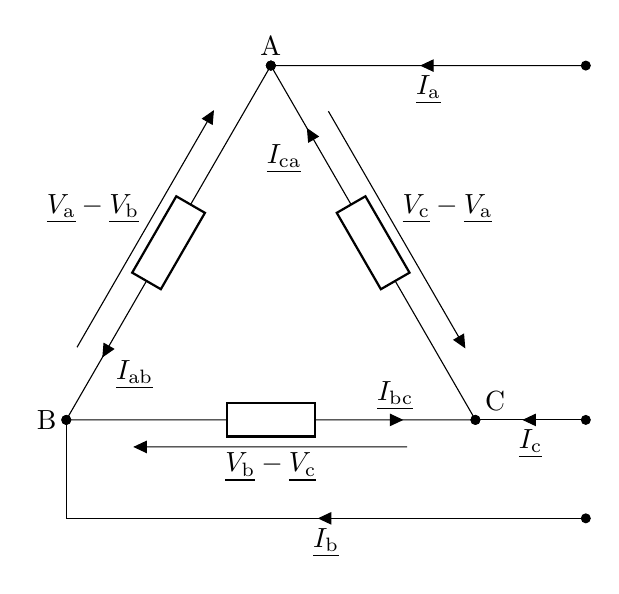
\begin{tikzpicture}[%
    show background rectangle,%
    tight background,%
    background rectangle/.style={fill=white}%
    ]
  \def\radius{2.3}%
  \def\Radius{3}%
  \ctikzset{bipoles/open/voltage/distance from node/.initial=0.1}%

  % Coordonnées
  \coordinate (A) at (90:\Radius);%
  \coordinate (B) at (210:\Radius);%
  \coordinate (C) at (330:\Radius);%
  \coordinate (A2) at ($(\Radius,\Radius)+(1,0)$);%
  \coordinate (C2) at (A2 |- B);%
  \coordinate (B2) at ($(C2)-(0,1.25)$);%
  \coordinate (B3) at ($(B)-(0,1.25)$);%

  % Nœuds
  \node[above] at (A) {A};%
  \node[left] at (B) {B};%
  \node[above right] at (C) {C};%

  % Lignes
  \draw (A) to[ generic, v<=$\underline{V_{\arm}}-\underline{V_{\brm}}$, i=$\underline{I_{\abrm}}$,
  *-*] (B) to[ generic, v<=$\underline{V_{\brm}}-\underline{V_{\crm}}$, i=$\underline{I_{\bcrm}}$,
  *-*] (C) to[ generic, v<=$\underline{V_{\crm}}-\underline{V_{\arm}}$, i=$\underline{I_{\carm}}$,
  *-*] (A);%
  \draw (A2) to[short,i=$\underline{I_{\arm}}$,*-*] (A);%
  \draw (B) -- (B3);%
  \draw (B2) to[short,i=$\underline{I_{\brm}}$,*-] (B3);%
  \draw (C2) to[short,i=$\underline{I_{\crm}}$,*-] (C);%
\end{tikzpicture}
\end{document}
% Local Variables:
% mode: latex
% TeX-engine: luatex
% TeX-source-correlate-method-active: synctex
% ispell-local-dictionary: "british"
% coding: utf-8
% LaTeX-indent-level: 4
% fill-column: 100
% End:
